\documentclass{beamer}
%
% Choose how your presentation looks.
%
% For more themes, color themes and font themes, see:
% http://deic.uab.es/~iblanes/beamer_gallery/index_by_theme.html
%
\mode<presentation>
{
  \usetheme{Boadilla}      % or try Darmstadt, Madrid, Warsaw, ...
  \usecolortheme{beaver} % or try albatross, beaver, crane, ...
  \usefonttheme{default}  % or try serif, structurebold, ...
  \setbeamertemplate{navigation symbols}{}
  \setbeamertemplate{caption}[numbered]
  
} 

\usepackage{xcolor,colortbl}
\usepackage[english]{babel}
\usepackage[utf8x]{inputenc}
\usepackage{courier}
\usepackage{dsfont}
\usepackage{verbatim} 
\usepackage{enumerate}
\usepackage{tikz}
\usepackage{multirow}
\usepackage{venndiagram}
\usepackage{epigraph} 
%\usepackage{xcolor}
\usepackage{makecell}

%\usepackage{enumitem}

\usepackage{hyperref}
\hypersetup{
    colorlinks=true,
    linkcolor=blue,
    filecolor=magenta,      
    urlcolor=cyan,
}

% R stuff!
\usepackage{listings}
\definecolor{codegreen}{rgb}{0,0.6,0}
\definecolor{codegray}{rgb}{0.5,0.5,0.5}
\definecolor{codepurple}{rgb}{0.58,0,0.82}
\definecolor{backcolour}{rgb}{0.95,0.95,0.92}

\lstdefinestyle{mystyle}{
    backgroundcolor=\color{backcolour},    
    commentstyle=\color{codegreen},
    keywordstyle=\color{black},
    numberstyle=\tiny\color{codegray},
    stringstyle=\color{codepurple},
    basicstyle=\ttfamily\footnotesize,
    breakatwhitespace=false,         
    breaklines=true,                 
    captionpos=b,                    
    keepspaces=true,                 
    numbers=left,                    
    numbersep=5pt,                  
    showspaces=false,                
    showstringspaces=false,
    showtabs=false,                  
    tabsize=2
}

\lstset{style=mystyle}


\setbeamertemplate{enumerate items}[default]
\setbeamertemplate{itemize item}[triangle]

%\setitemize{label=\usebeamerfont*{itemize item}%
%  \usebeamercolor[fg]{itemize item}
%  \usebeamertemplate{itemize item}}



\title[Introduction to Statistics]{Normal Distributions}
\subtitle{}
\author{Grinnell College}
\date{October 14, 2024}

\graphicspath{{img/}}

\begin{document}

\begin{frame}
  \titlepage
\end{frame}

\begin{frame}{Review -- Inference}
\begin{center}
\usetikzlibrary{decorations.pathreplacing,positioning, arrows, shapes, calc,shapes.multipart}
\tikzstyle{block1} = [rectangle, draw, fill=yellow!20, 
    text width=10em, text centered, rounded corners, minimum height=6em]
\tikzstyle{block2} = [rectangle, draw, fill=yellow!20, 
    text width=5em, text centered, rounded corners, minimum height=3em]
\tikzset{
    %Define standard arrow tip
    >=stealth,
    % Define arrow style
    pil/.style={
           ->,
           thick,
           shorten <=2pt,
           shorten >=2pt,}
}
\tikzstyle{line} = [draw, -latex]
\begin{tikzpicture}[node distance = 3cm, auto]
            % Place nodes
            \node [block1] (pop) {Population \\ (Parameter)};
            \node [block2, below of=pop] (samp) {Sample \\ (Statistic)};
            
            % Draw edges
            \draw[<-, >=latex, shorten >=2pt, shorten <=2pt, bend right=45, thick]  (pop.west) to node[auto, swap] {Inference}(samp.west);
            \draw[<-, >=latex, shorten >=2pt, shorten <=2pt, bend right=45, thick] (samp.east) to node[auto, swap] {Study Design}(pop.east); 
            
        \end{tikzpicture}
  \end{center}
\textbf{BIG IDEA:} Parameter value is unknown $\rightarrow$ we use the statistic to estimate it  
\end{frame}

\begin{frame}{Review -- Sampling Distribution}
If we had the ability to make many different samples we could plot the statistics from each.
\begin{itemize}
    \item This gives us an idea of the variability of the statistics
\end{itemize}

\begin{center}
    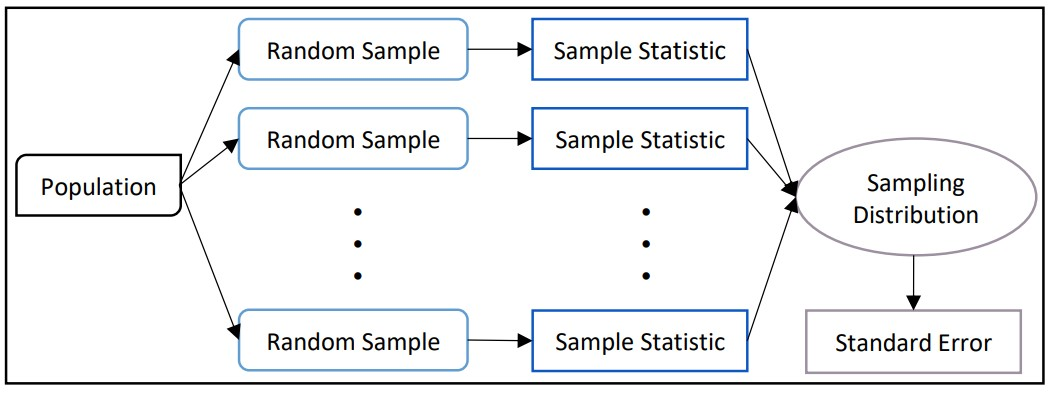
\includegraphics[scale=.5]{img/sampling_distr_method.jpg}
\end{center}
The \textbf{Standard Error} is the std. dev. of the sampling distribution
\begin{itemize}
    \item measures variability of statistics
\end{itemize}
\end{frame}

\begin{frame}{Sampling Distribution}
To make the sampling distribution, we had to take a whole lot of different samples.
\begin{itemize}
    \item Are there any issues with this?
    \item Would you actually want to go and take 5,000 different samples?
\end{itemize}
\end{frame}

\begin{frame}{What now?}
Ok, so we can't just go and take a whole bunch of random samples... \vspace{10mm}

This means we can't get the standard error!
\begin{itemize}
    \item so we can't actually quantify how far the statistic away is? Wasn't that the whole point?!
\end{itemize} \vspace{10mm}

What the heck do we do now?
\end{frame}

\begin{frame}{Sampling Distribution Shape}
All hope is not lost. Think back to the shape of the sampling distribution. \vspace{15mm}

Big question: What happened to the shape of the sampling distribution as the sample size increased?
\end{frame}

\begin{frame}{Movie Budgets Example}
\begin{center}
    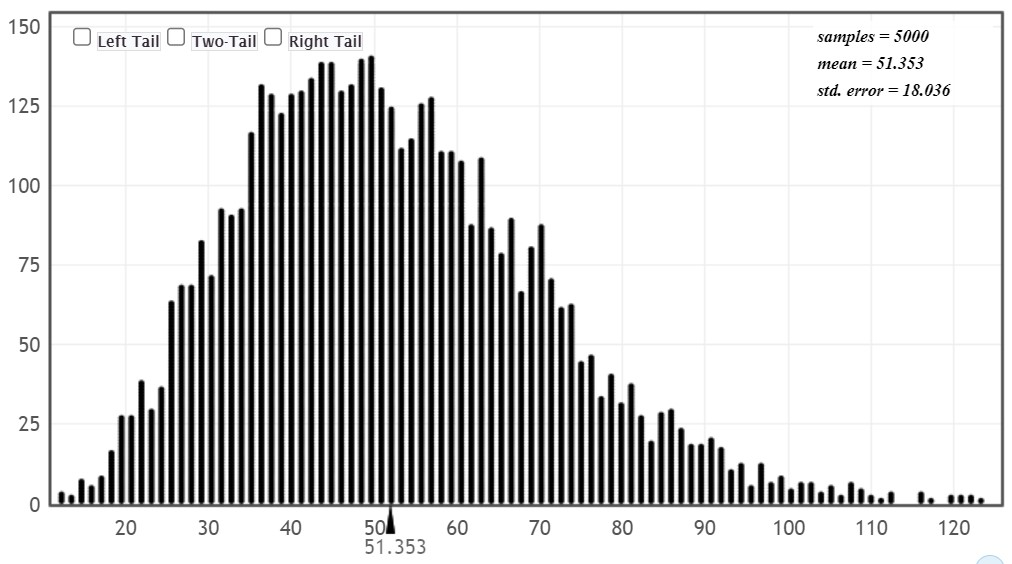
\includegraphics[scale=.4]{img/budgets_n10.jpg}
    
    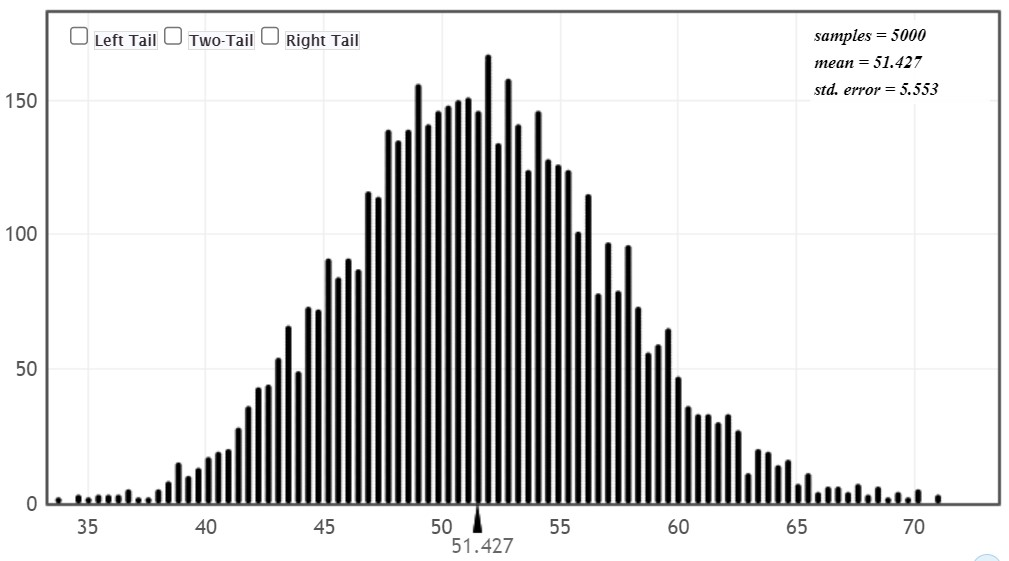
\includegraphics[scale=.4]{img/budgets_n100.jpg}
\end{center}
\end{frame}

\begin{frame}{Bell-shaped Distribution}
\begin{center}
    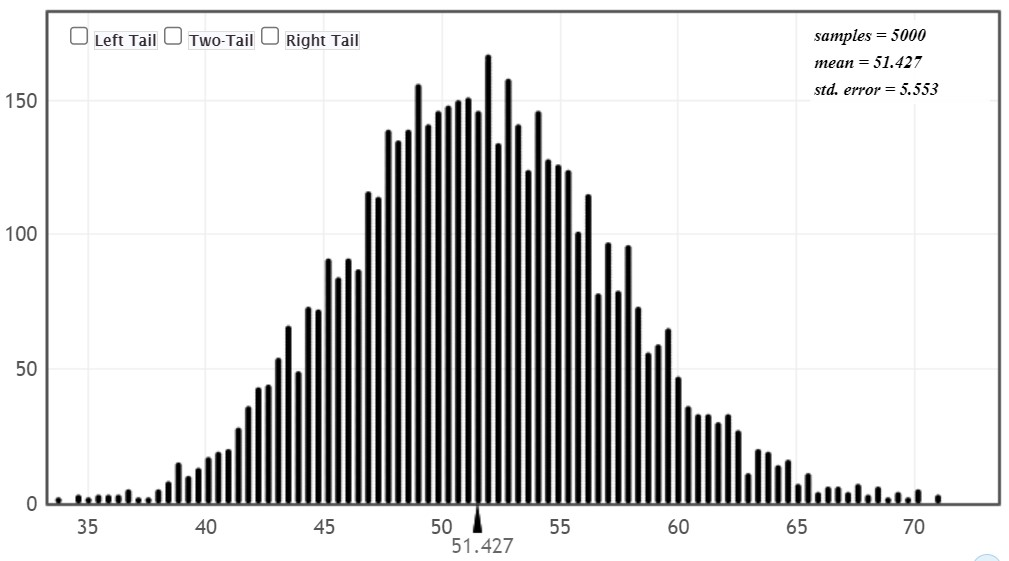
\includegraphics[scale=.4]{img/budgets_n100.jpg}
\end{center}

The bell-shaped distribution we see in the sampling distribution for Movie Budgets is something that happens a lot. \vspace{6mm}

It turns out there is a reason for that, which we will cover shortly. \vspace{6mm}

For now, we are going to give it a special name, and see what we can do with it.
\end{frame}

\begin{frame}{The Normal Distribution}

\begin{center}
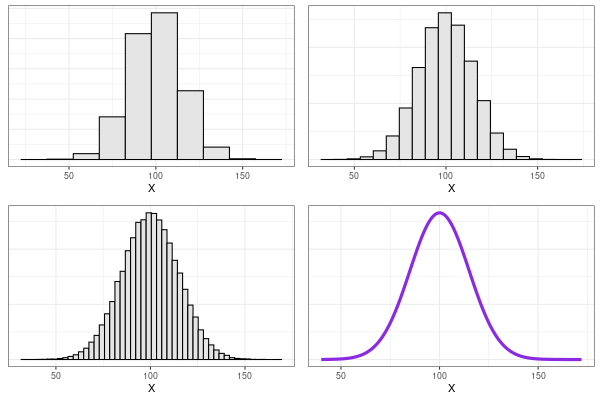
\includegraphics[scale=0.45]{normal_hist.png}
\end{center}
\end{frame}

\begin{frame}{Normal Distribution}
It turns out we only need to know two things in order to completely describe the Normal distribution
\begin{enumerate}
    \item the mean ($\mu$)
    \item the standard deviation ($\sigma$) \underline{or} variance ($\sigma^2$)
\end{enumerate} \vspace{4mm}

These will tell us where the center of the normal distribution is and how stretched out it should be. \vspace{4mm}

If a variable looks like a normal distribution, we will often use the following notation to say that:
\begin{itemize}
    \item X $\sim$ N($\mu$, $\sigma^2$)
\end{itemize}
\end{frame}

\begin{frame}{Normal Distribution}
X $\sim$ N($\mu$, $\sigma^2$)
\begin{itemize}
    \item the \underline{mean} tells us where the center of the normal distribution is
    \item the \underline{variance} tells us how spread out the distribution is
\end{itemize}
\begin{center}
    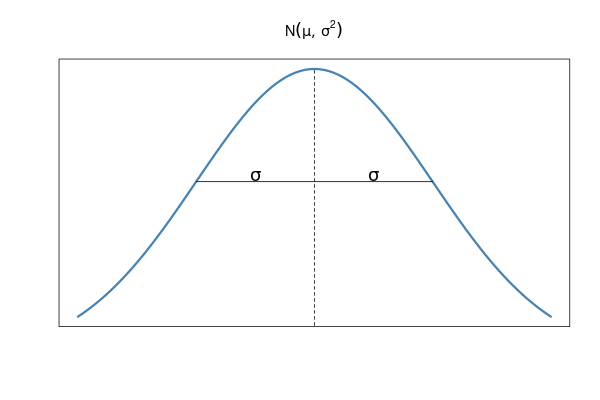
\includegraphics[scale=.4]{img/normal_pars.png}
    \vspace{-12mm}
    
    \hspace{2.5mm}$\mu$
\end{center}
\end{frame}

\begin{frame}{Examples}
\begin{center}
    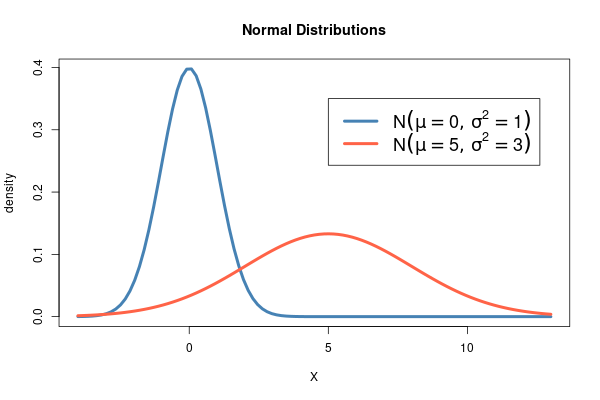
\includegraphics[scale=.55]{img/two_normals.png}
\end{center}
\end{frame}

\begin{frame}{Standard Normal Distribution}
When a normal distribution has mean zero and variance equal to 1, we call it a \textbf{Standard Normal Distribution} and write X $\sim$ N(0, 1). \vspace{4mm}

Why? It's related to standardizing variable like we did with Z-scores. \vspace{12mm}

Suppose the variable X $\sim$ N($\mu$, $\sigma^2$), 

then $Y = \frac{X-\mu}{\sigma} \sim$ N($\mu=0$, $\sigma^2=1$) \vspace{6mm}

In other words, if we standardize a normal variable (with any mean and variance) then we get back a normal variable that has $\mu = 0$ and $\sigma^2=1$
\end{frame}

\begin{frame}{Probabilities}
\textbf{Probabilities}

If our population follows a normal distribution... we can pick a case at random from our population
\begin{itemize}
    \item probability the observation is less/greater than some value?
    \item probability the observation is between two values?
\end{itemize} \vspace{10mm}

\textbf{Note:} It turns out that using a normal distribution we cannot find the probability of the case having a *specific* value, we can only use ranges of values.
\end{frame}

\begin{frame}{Probabilities -- Less than}
Standard Normal: X $\sim$ N(0, 1)

Probability a randomly selected observation is below (less than) \textbf{-1}?
\begin{center}
    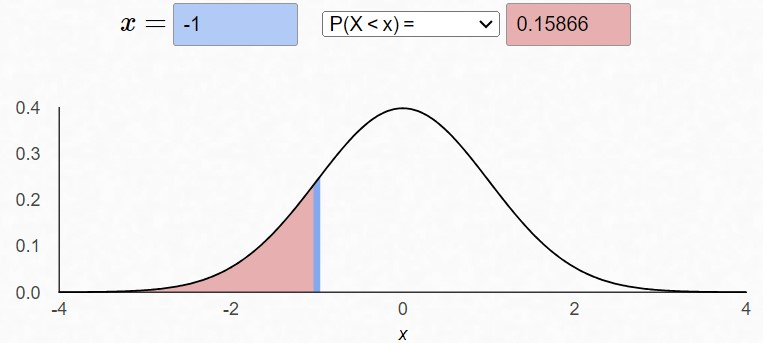
\includegraphics[scale=.7]{img/norm_prob1.jpg}
\end{center}
We can write this using our probability notation: P(X $<$ -1) = 0.15866

\end{frame}

\begin{frame}{Probabilities -- Greater than}
Standard Normal: X $\sim$ N(0, 1)

Probability a randomly selected observation is above (greater than) \textbf{0.43}?
\begin{center}
    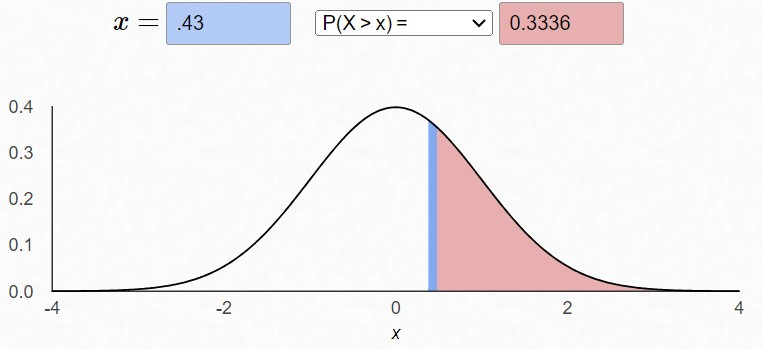
\includegraphics[scale=.7]{img/norm_prob2.jpg}
\end{center}
P(X $>$ 0.43) = 0.3336
\end{frame}

\begin{frame}{Probabilities -- Between}
Standard Normal: X $\sim$ N(0, 1)

What about the probability that a case falls \textit{between} \textbf{-1} and \textbf{1}?
\begin{center}
    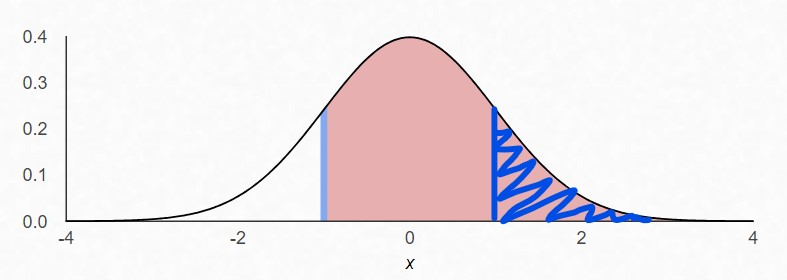
\includegraphics[scale=.7]{img/norm_prob3.jpg}
\end{center}
We need to do a bit more work...
\end{frame}

\begin{frame}{Probabilities -- Between}
Standard Normal: X $\sim$ N(0, 1)

What about the probability that a case falls \textit{between} \textbf{-1} and \textbf{1}? \vspace{8mm}

\begin{columns}
 \begin{column}{0.37\textwidth}
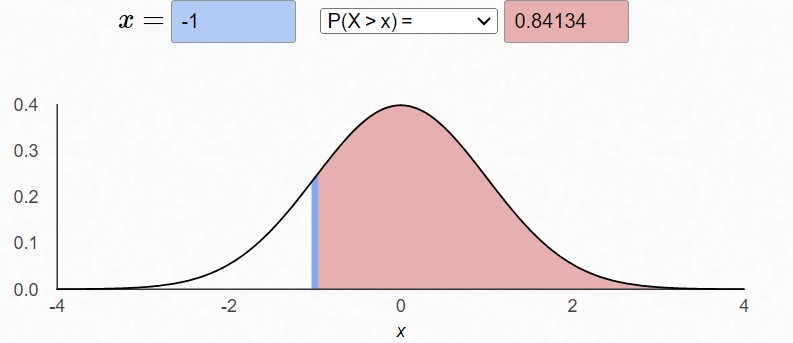
\includegraphics[scale=.38]{img/norm_prob4.jpg}
 \end{column}
 \begin{column}{0.37\textwidth}
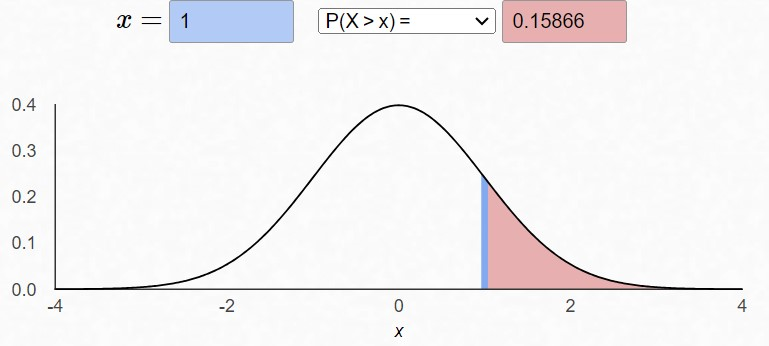
\includegraphics[scale=.38]{img/norm_prob5.jpg}
 \end{column}
\end{columns}

We can chop off the extra probability we don't need that is above \textbf{1}. \vspace{8mm}

P(X is between -1 and 1) = P(-1 $<$ X $<$ 1) = P(X $<$ -1) - P(X $<$ 1)

\hspace{41mm} = 0.84134 - 0.15866 = 0.68286
\end{frame}


\begin{frame}{Probabilities -- Between}
When the values we are looking at are the same but just with different signs (like -1 and +1)
\begin{itemize}
    \item We can write them in a specific way
    \item There is a shortcut on the app for getting the probability
\end{itemize}
\end{frame}

\begin{frame}{Probabilities -- Between}
Standard Normal: X $\sim$ N(0, 1)

What about the probability that a case falls \textit{between} \textbf{-1} and \textbf{1}?
\begin{center}
    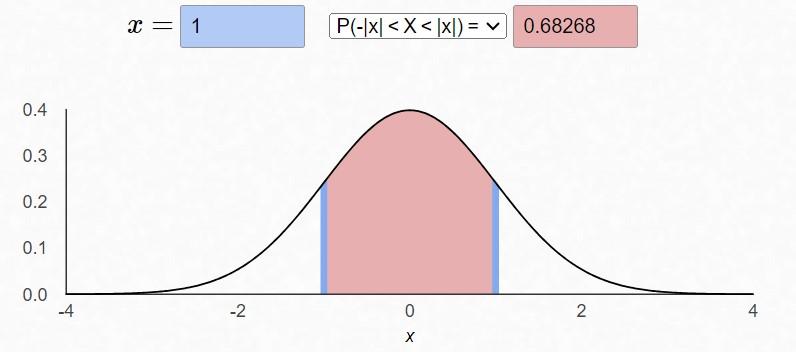
\includegraphics[scale=.7]{img/norm_prob6.jpg}
    
    P($|X| <$ 1) = 0.68286
\end{center}
\end{frame}

\begin{frame}{Probabilities -- Between}
Standard Normal: X $\sim$ N(0, 1)

What about the probability that a case falls \textit{between} \textbf{-2} and \textbf{2}?
\begin{center}
    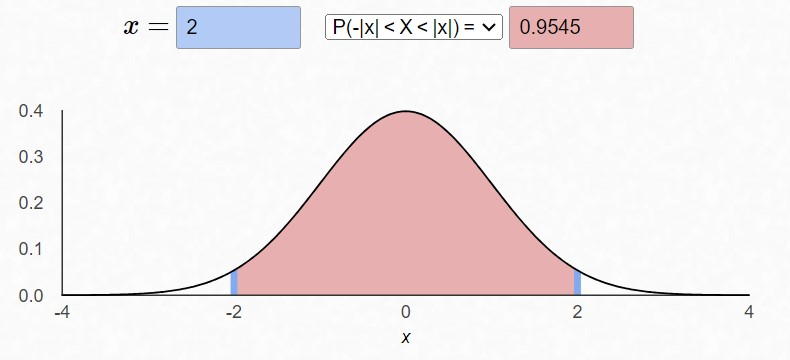
\includegraphics[scale=.7]{img/norm_prob7.jpg}

    P($|X| <$ 2) = 0.9545
\end{center}
\end{frame}

\begin{frame}{Probabilities -- Between}
Standard Normal: X $\sim$ N(0, 1)

What about the probability that a case falls \textit{between} \textbf{-1} and \textbf{1}?
\begin{center}
    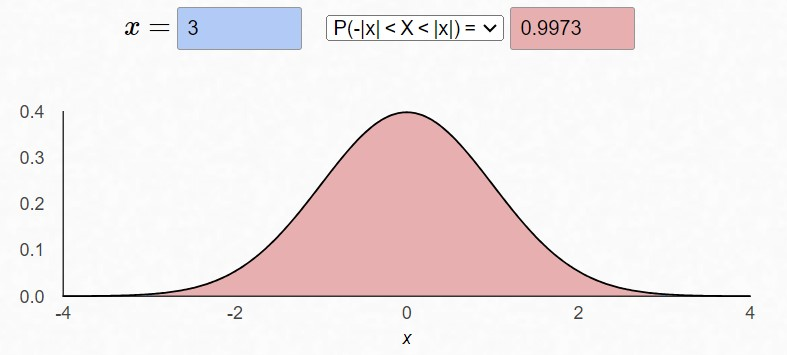
\includegraphics[scale=.7]{img/norm_prob8.jpg}

    P($|X| <$ 3) = 0.9973
\end{center}
\end{frame}

\begin{frame}{Summary}
\begin{center}
    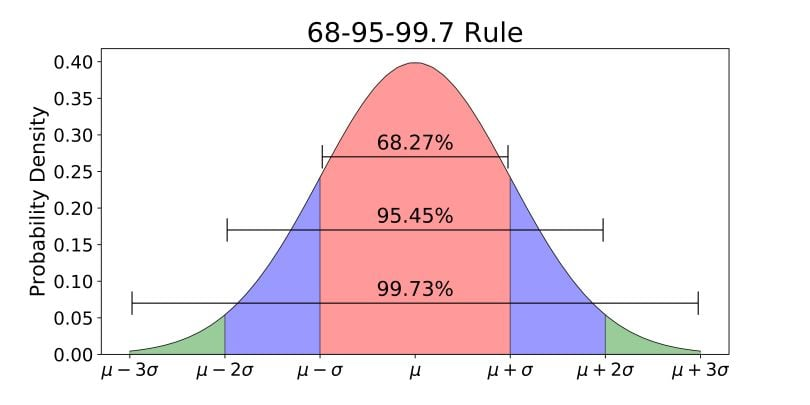
\includegraphics[scale=.45]{img/empirical_rule.jpg}
\end{center}
\end{frame}

\begin{frame}{Probabilities from R}
We can use the "pnorm()" function in R to get these probabilities.
\begin{itemize}
    \item tell the function what number you are trying to find the probability more/less than
    \item tell the function the value of the mean
    \item tell the function the value of the std. dev.
\end{itemize} \vspace{2mm}

\scriptsize{\textbf{Note:} By default R will try to give you 'less than' probabilities (also called lower tail probabilities). To get 'greater than' probabilities, put "Lower.Tail=FALSE" into the pnorm() function.} \vspace{2mm}

\begin{center}
    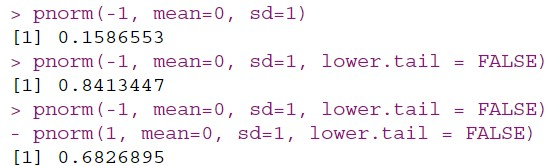
\includegraphics[scale=1]{img/pnorm_R_example.jpg}
\end{center}
\end{frame}

\begin{frame}{Central Limit Theorem}
The \textbf{Central Limit Theorem (CLT)} is (possibly) the most important result in all of statistics. It states:
\begin{enumerate}
    \item If variable X has mean $\mu$ and std.dev. $\sigma$, and
    \item If the number of observations in the sample (n) is large
    \item then the sampling distribution for $\overline{X}$ (sample mean) is Normal with mean $\mu$ and standard error $\sigma / \sqrt{n}$.
\end{enumerate}
\begin{center}
    $\overline{X} \sim$ N($\mu$, $\sigma^2 / n$)
\end{center}
\end{frame}

\begin{frame}{Central Limit Theorem}
    \textbf{Important bits}:

\begin{itemize}
    \item CLT doesn't require the pop. distribution look Normal \vspace{4mm}
    \item What is considered large?
    \begin{itemize}
        \item A recommendation for being “sufficiently large” when working with means is often to have at least 30 cases in your sample \vspace{3mm}
        \item If the data are approximately normal or symmetric, a smaller sample size (10 to 20) may be sufficient  \vspace{3mm}
        \item If the data are skewed and/or have extreme outliers, the sample size may need to be higher than 30; possible more than 45. If the skew and outliers are very extreme, the sample size may need to be higher than around 200
    \end{itemize}
\end{itemize}
\end{frame}

\begin{frame}{Summary}
We learned a bit about the Normal distribution!
\begin{itemize}
    \item what it looks like
    \item how to find probabilities with it
    \item how it relates to the sampling distribution (CLT)
\end{itemize} \vspace{6mm}

\textbf{Central Limit Theorem} tells us that for large samples $\overline{X} \sim$ N($\mu$, $\sigma^2 / n$) \vspace{6mm}

We don't need to take 5,000 samples to get the \textbf{Standard Error} any more! We have a formula:
\begin{itemize}
    \item SE = $\sigma / \sqrt{n}$
\end{itemize}


\end{frame}



%%%%%%%%%%%%%%%%

%\begin{frame}
%\begin{columns}
%
%  \begin{column}{0.45\textwidth}
%%
%  \end{column}
%  \begin{column}{0.45\textwidth}
%%
%  \end{column}
%
%\end{columns}
%\end{frame}


\end{document}

